% (c) 2015 Daniele Zambelli daniele.zambelli@gmail.com

\chapter{Geometria nello spazio}

\section{TODO}

\section{Assiomi}
\label{sec:3D_assiomi}

% \begin{wrapfloat}{figure}{r}{0pt}
% \includegraphics[scale=0.35]{img/fig000_.png}
% \caption{...}
% \label{fig:...}
% \end{wrapfloat}
% 
% \begin{center} \input{\folder lbr/fig000_.pgf} \end{center}

\section{Vettori geometrici e vettori applicati}

In questa sezione vogliamo richiamare il concetto di vettore geometrico e 
fornire
un significato ``rigoroso'' al concetto di vettore applicato, essenziali per le 
applicazioni 
fisica e in particolare per la meccanica razionale. 

\begin{definition}
  Un {\bf segmento orientato} \`e un segmento in cui sia stato scelto un ordine 
tra i due
  estremi ed \`e quindi individuato da una coppia ordinata di punti. Il primo 
punto \`e detto
  {\it coda} o {\it origine} e il secondo \`e detto {\it punta}  o {\it fine}. 
  Un segmento orientato, rappresentato in figura (graficamente con una 
freccia), 
  \`e denotato dai punti di estremo: l'origine seguita dalla punta.
%%% ========================= FIGURE  ======================
\begin{figure}[h!]
\begin{center}
{\small
{\scalebox{.7}{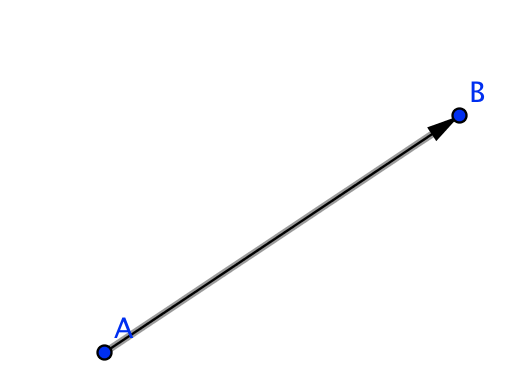
\includegraphics{vettore}}}
%\put(-132,-5){$\frac{1}{2}$}
%\put(-42,75){$\frac{1}{2}$}
}
%\caption{\small }\label{fig:???}
\end{center}
\end{figure}
%%% =======================================================    
\end{definition}

I segmenti orientati $AB$ e $BA$ contengono lo stesso insieme di punti, ma sono 
diversi, 
essendo diverso l'ordine degli estremi. Ogni punto individua un segmento banale 
in cui origine 
e fine coincidono. Un segmento orientato definisce tre grandezze:
\begin{itemize}
  \item \textcolor{red}{\bf direzione:} retta (o pi\`u propriamente un fascio di 
rette) contenente $AB$;
  \item \textcolor{red}{\bf verso:} $A$ precede $B$;
  \item \textcolor{red}{\bf lunghezza:} una volta fissata una unit\`s di misura 
questa determina 
  la lunghezza del vettore. Ovviamente $AA$ ha lunghezza nulla.
\end{itemize}

\begin{definition}
  Due segmenti orientati $AB$ e $CD$ si dicono {\bf equipollenti} se hanno la 
stessa
  lunghezza, la stessa direzione e lo stesso verso e si pone $AB\equiv CD$. 
\end{definition}

La relazione di equipollenza \`e una relazione di equivalenza, ossia si ha che 
1. ogni segmento
orientato \`e equipollente a se stesso ({\it riflessivit\`a}); 
2. se $AB$ \`e equipollente a $CD$ allora anche $CD$ \`e
equipollente ad $AB$ ({\it simmetria}); 
3. se $AB$ \`e equipollente ad $CD$ e $CD$ \`e equipollente a $EF$,
allora anche $AB$ \`e equipollente a $EF$ ({\it transitivit\`a}). 
Da ci\`o si deduce che l'insieme dei segmenti
orientati \`e suddiviso (o meglio {\it partizionato}) in classi di equipollenza 
a due a due
disgiunte: cio\`e \`e sempre possibile stabilire se un segmento orientato 
appartiene o meno
ad una determinata classe e esso appartiene solo ad una classe. La propriet\`a 
appena 
osservata permette di definire il concetto di vettore geometrico.
\begin{definition}
  Chiamiamo {\it vettore geometrico} una classe di equipollenza di segmenti 
orientati. 
  L'insieme $\bS{}$ di tali classi \`e detto {\bf spazio vettoriale geometrico}.
\end{definition}

Mostriamo ora che $\bS{}$ \`e effettivamente un  $\bR{}$--spazio vettoriale. 
Notiamo che ha senso parlare 
di lunghezza, direzione e verso di un vettore geometrico,\footnote{D'ora in poi 
scrivere semplicemente vettore invece che vettore geometrico.} considerando 
quelle di uno 
qualsiasi dei suoi rappresentanti. La classe dei segmenti orientati banali 
definisce il vettore
nullo $\vec 0$, inoltre due vettori si dicono opposti se hanno uguale direzione 
e lunghezza 
ma verso opposto e infine due vettori si dicono paralleli se hanno la stessa 
direzione.

Introduciamo ora le due operazioni che renderanno $\bS{}$ un $\bR{}$--spazio 
vettoriale. 

\begin{itemize}
  \item {\bf Somma tra vettori.}\footnote{Metodo punta--coda o del 
parallelogramma.} 
  Consideriamo due vettori $\vec v$ e $\vec w$. La somma
  $\vec v+\vec w$ si effettua seguendo i seguenti passi:
  \begin{itemize}
    \item[i.] si scelga un punto $A$;
    \item[ii.] si scelgano altri due punti $B$ e $C$ in modo che $AB = \vec v$ e 
$BC = \vec w$;
    \item[iii.] $\vec v+\vec w := AC$, cio\`e definiamo la somma di $\vec v$ con 
$\vec w$ come
    la classe di equipollenza di segmenti orientati di rappresentante il 
segmento orientati
    $AC$. 
  \end{itemize}
  \item {\bf Prodotto per scalari.} Siano $\vec v\in\bS{}$ e $\alpha\in\bR{}$. 
Il vettore 
  $\vec w: = \alpha \,\vec v$ \`e il vettore diretto come $\vec v$ di lunghezza 
pari a 
  $|\alpha|\, \|\vec v\|$ e di verso concorde a $\vec v$ se $\alpha>0$, discorde 
se $\alpha<0$, 
  inoltre se $\alpha = 0$, $\vec w = \vec 0$. 
\end{itemize}
Tali operazioni soddisfano le propriet\`a a cui devono soddisfare l'operazione 
interna 
e il prodotto per scalari nel caso degli spazi vettoriali (si verifichi per 
esercizio), 
cio\`e $\bS{}$ dotato di queste due operazioni \`e un $\bR{}$--spazio 
vettoriale.\\

Definiamo ora cosa significa applicare un vettore ad un punto; operazione 
fondamentale 
in fisica. L'operazione di applicazione di un vettore ad un punto $P$ consiste 
nello scegliere
quel particolare segmento orientato della classe, cio\`e quel determinato 
rappresentante,
avente origine in $P$: un vettore applicato consiste quindi di una coppia 
$(P,\vec v)$, 
in cui $P\in\bA{3}$ e $\vec v\in \bS{}$. L'insieme dei vettori applicati ad un 
punto prefissato $A$
viene denotato con $\bS{}_A$ ed \`e dotato della struttura di $\bR{}$--spazio 
vettoriale. 
Un vettore applicato in un punto $A$ si pu\`o scrivere:
\[
  B = A+\vec v \quad \textrm{ oppure }\quad  \vec v= B-A.
\]
Inoltre $\bS{}_A$ \`e banalmente isomorfo allo spazio dei segmenti orientati con 
origine in $A$.
\`E ora abbastanza semplice costruire un isomorfismo tra lo spazio dei vettori 
geometrici
$\bS{}$ e lo spazio dei vettori applicati $\bS{A}$ in un punto fissato $A$: \`e 
sufficiente
introdurre un sistema di riferimento con origine in $A$ e applicare poi i 
vettori all'origine.
Cos\`{i} facendo si identificano i vettori $\vec v:= AP$ con le coordinate dei 
punti di punta $P$
\[
  \vec v_0 \longmapsto \begin{bmatrix} x_0\\y_0\\z_0 \end{bmatrix}
\]
e le operazioni appena introdotto divengono operazioni tra le coordinate.

%%% ========================= FIGURE  ======================
\begin{figure}[h!]
\begin{center}
{\small
{\scalebox{.7}{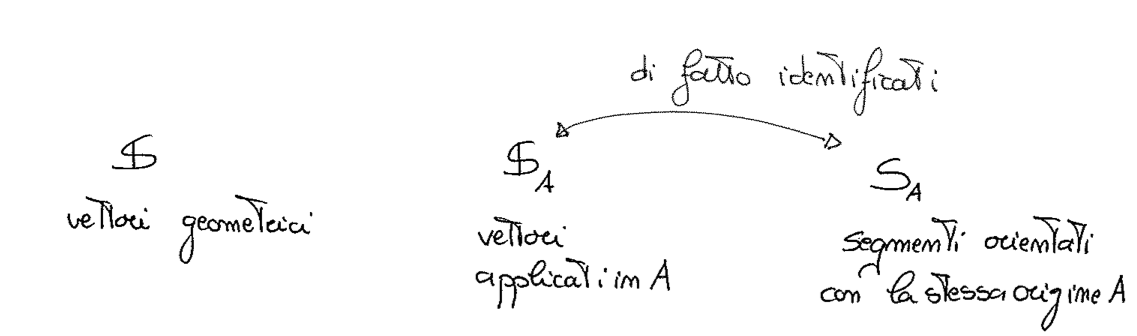
\includegraphics{isomorfismo}}}
%\put(-132,-5){$\frac{1}{2}$}
%\put(-42,75){$\frac{1}{2}$}
}
%\caption{\small Interpretazione geometrica del prodotto misto}%\label{fig:???}
\end{center}
\end{figure}
%%% =======================================================    

\begin{NB}
  Si noti, per\`o, che l'isomorfismo appena introdotto non \`e canonico, cio\`e 
dipende 
  dalla scelta del sistema di riferimento, mentre le operazioni tra i vettori 
sono definite
  intrinsecamente! La natura geometrica dei vettori permette di scegliere in 
ogni 
  occasione il sistema di riferimento pi\`u opportuno. Questo fatto \`e di 
fondamentale 
  importanza in meccanica, perche`, assieme ai principi di Newton emerge 
chiaramente
  che il sistema di riferimento (purch\'e inerziale) pu\`o essere scelto in modo 
arbitrario.
\end{NB}

La costruzione introdotta permette di affermare che l'insieme dei vettori 
geometrici pu\`o 
essere dotato di una struttura affine. Ricordiamo che una delle differenze 
fondamentali
tra spazi vettoriali e spazi affini \`e che mentre in uno spazio vettoriale 
l'origine dei sistemi
di riferimento \`e necessariamente il vettore nullo, in uno spazio affine 
l'origine pu\`o
essere posta in qualsiasi punto.

\section{Struttura euclidea dello spazio dei vettori geometrici}
Lo spazio dei vettori geometrici, per\`o, non solo \`e dotato della struttura 
affine, 
ma anche della struttura euclidea ereditata dalla struttura euclidea standard di
$\bR{3}$. Siano $\vec v$ e $\vec w$ due vettori di $\bS{}$ in cui sia stato 
introdotto 
un sistema di riferimento, ossia sia stato fissato un punto $O$ detto {\it 
origine} e 
sia stati scelti tre vettori linearmente indipendenti (formanti una base di 
$\bR{3}$).
Siano quindi $[v_1\quad v_2\quad v_3]^T$ e $[w_1\quad w_2\quad w_3]^T$ le 
coordinate
di $\vec v$ e $\vec w$, rispettivamente. 

\begin{definition}
  Il prodotto scalare euclideo di $\bS{}$ \`e l'applicazione bilineare, 
simmetrica 
  e definita positiva
  \[\begin{aligned}
    \cdot : & \; \bS{}\times\bS{} \longrightarrow \bR{} \\
         & \; (\vec v,\vec w) \longmapsto \vec v\cdot \vec w := v_1\,w_1 + 
v_2\,w_2 + v_3\,w_3 
         = \sum_{j=1}^3 v_j\,w_j
  \end{aligned}\]
\end{definition}

\begin{itemize}
  \item {\bf bilineare}: lineare in entrambe le entrate del prodotto; 
  \item {\bf simmetrica}: $\vec v\cdot \vec w = \vec w = \vec v$;
  \item {\bf definita positiva}: $\vec v\cdot \vec v \ge 0$ e l'uguaglianza vale 
se e solo se 
            $\vec v = \vec 0$.
\end{itemize}
Lo spazio dei vettori geometrici (ma pi\`u in generale lo spazio affine $\bA{3}$ 
3--dimensionale 
a lui isomorfo) munito di un prodotto scalare euclideo \`e detto {\bf spazio 
euclideo} 
3--dimensionale e si indica con $\bE{3}$.

La nozione di prodotto scalare permette di introdurre una nozione di lunghezza o 
norma 
di un vettore, usando le coordinate:
\[\begin{aligned}
  \|\cdot \| &\; \bS{} \longrightarrow \bR{}_+\\
  &\; \vec v \longmapsto := \|\vec v\| := \sqrt{\vec v\cdot \vec v}
\end{aligned}\]

\begin{proprieta}
  \begin{itemize}
    \item $\| \vec v \| = 0$ se e solo se $\vec v = \vec 0$;
    \item[]
    \item $\| \alpha\,\vec v\| = |\alpha|\, \|\vec v \|$ con $\alpha\in\bR{}$;
    \item[]
    \item $\| \vec v+\vec w \| \le \|\vec v\|\, \|\vec w\|$ (disuguaglianza 
triangolare);
    \item[]
    \item $\| \vec v+\vec w \|^2 = \|\vec v\|^2 + 2\, \vec v\cdot \vec w + 
\|\vec w\|^2$ (Teorema di Carnot);
    \item[]
    \item $\|\vec v+\vec w\|^2 + \|\vec v-\vec w\}^2 = 2\, \left(\|\vec v\|^2 
+\|\vec w\|^2 \right)$ 
    \item[]
    \item $|\vec v\cdot \vec w|\le\|\vec v\|\,\|\vec w\|$ (disuguaglianza di 
Cauchy--Schwarz).\footnote{Per esercizio dimostrare le propriet\`a qui 
elencate.}
  \end{itemize}
\end{proprieta}
La disuguaglianza di Cauchy--Schwarz assicura che
\[
  \frac{|\vec v\cdot \vec w|}{\|\vec v\|\, \|\vec w\|}\le 1,
\]
e ci\`o permette di introdurre il concetto di angolo o pi\`u precisamente 
di coseno di un angolo non orientato:
\[
  \cos\theta(\vec v,\vec w) = \frac{|\vec v\cdot \vec w|}{\|\vec v\|\, \|\vec 
w\|};
\]
recuperando cos\`{i} anche la nozione di prodotto scalare nota dalla fisica.
La nozione di angolo consente di introdurre il concetto di ortogonalit\`a tra 
vettori. Precisamente 
\begin{definition}   
  Due vettori $\vec v$, $\vec w$ di $\bS{}$ si diranno {\it ortogonali} 
  \[
    \vec v\cdot \vec w = 0.
  \]
\end{definition}  
Inoltre, come noto dai corsi di Algebra lineare e Geometria (analitica), due 
vettori 
ortogonali sono linearmente indipendente, inoltre in uno spazio euclideo \`e 
possibile
definire una base ortogonale o ortonormale (in quest'ultimo caso i vettori di 
base oltre ad
essere a due a due ortogonali devono avere norma unitaria\footnote{Un vettore 
di 
norma unitaria \`e anche detto versore.}). Tranne in alcuni 
casi espressamente indicati lavoreremo con basi ortogonali in $\bE{3}$, 
denotando con
$\{e_1,e_2,e_3\}$ o $\{c_1,c_2,c_3\}$ o $\{i,j,k\}$ e versori di base.
\begin{example}
  {\it Verificare che i vettori $\vec v= [1\quad 0 \quad -1]^T$ e $\vec w = 
[2\quad 0 \quad 2]^T$
  sono ortogonali ma non sono versori.}
\end{example}
\begin{sol}
  {\it Osserviamo che $\vec v\cdot \vec w = 2+0-2 = 0$, per cui $\vec v$ e $\vec 
w$
  sono ortogonali. La norma di $\vec v$ \`e $\|\vec v\| = \sqrt{\vec v\cdot \vec 
v} = \sqrt 2$,
  mentre la norma di $\vec w$ \`e $\|\vec w\| = \sqrt{\vec w\cdot \vec w} = 
2\sqrt 2$. } 
\end{sol}

Ora, dato un vettore non nullo $\vec v$ \`e sempre possibile costruire un 
versore avente 
stessa direzione e stesso verso: \`e sufficiente dividere il vettore originario
per la sua norma:
\[
  \vec u := \frac{\vec v}{\|\vec v\|}.
\]
Infatti
\[
  \vec u\cdot \vec u = \frac{\vec v}{\|\vec v\|}\cdot \frac{\vec v}{\|\vec v\|} 
  = \frac{1}{\|\vec v\|^2}\, \vec v\cdot \vec v = \frac{\|\vec v\|^2}{\|\vec 
v\|^2} = 1.
\]
\begin{example}
  {\it Con riferimento all'esempio precedente normalizzare i vettori $\vec v$ e 
$\vec w$
  e completarli ad una base ortonormale di $\bE{3}$.}
\end{example}
\begin{sol}
  Poniamo
  \[
  \vec b_1 = \frac{\vec v}{\|\vec v\|} = \frac{\sqrt 2}{2} \begin{bmatrix} 
1\\0\\-1 \end{bmatrix}
  \textrm{ e } 
  \vec b_2 \frac{\vec w}{\|\vec w\|} = \frac{\sqrt 2}{8} \begin{bmatrix} 2\\0\\2 
\end{bmatrix}\]
  
  che sono ortonormali. Per completare $b_1$ e $b_2$ ad una base ortonormale di 
  $\bE{3}$ \`e sufficiente aggiungere il vettore $e_2$.
  
  In caso non ci si accorgesse di tale fatto, bisognerebbe scrivere un qualche 
vettore 
  linearmente indipendente da $\vec b_1$ e $\vec b_2$ e poi applicargli la 
procedura 
  di ortonormalizzazione di Gram--Smith  per la quale si rimanda ad un libro di 
  Algebra Lineare e Geometria.
\end{sol}

\section{Prodotto vettoriale e prodotto misto}
Nello spazio euclideo {\bf 3--dimensionale} $\bE{3}$ oltre al prodotto scalare
rimane definito il prodotto  vettoriale di due vettori
\[\begin{aligned}
  \cdot \times \cdot : & \quad \bE{3}\times\bE{3} \longrightarrow \bE{3} \\
     & \quad (\vec v,\vec w) \longmapsto \vec v\times\vec w:=
     \begin{bmatrix} 
        v_2\,w_3 - v_3\,w_2 \\
        v_3\,w_1 - v_1\,w_3 \\
        v_1\,w_1-v_2\,w_1
     \end{bmatrix}
\end{aligned}\]     
in cui $\vec v = [v_1\quad v_2\quad v_3]^T$ e $\vec w = [w_1\quad w_2 \quad 
w_3]^T$.

Una formula utile per l'espressione del prodotto vettoriale consiste nel porre i 
vettori
$\vec v$ e $\vec w$, nell'ordine assegnato, come seconda e terza riga di una 
matrice
e come prima riga porre i vettori della base canonica:
\[\begin{bmatrix}
  i& j & k\\
  v_1 & v_2 & v_3\\
  w_1 & w_2 &w_3
\end{bmatrix}\]
e poi sviluppare come un determinante ma {\bf esclusivamente rispetto alla
prima riga}, ottenendo
\[\begin{bmatrix}
    i& j & k\\
    v_1 & v_2 & v_3\\
    w_1 & w_2 &w_3
  \end{bmatrix} = 
  \begin{bmatrix} 
        v_2\,w_3 - v_3\,w_2 \\
        v_3\,w_1 - v_1\,w_3 \\
        v_1\,w_1-v_2\,w_1
  \end{bmatrix}
\]
\begin{proprieta}
  \begin{itemize}
    \item $\vec v\times \vec w = - \vec w\times \vec v$;
    \item $(\vec v+\vec u)\times \vec w = \vec v\times \vec w + \vec u\times\vec 
w$;
    \item $(\lambda\, \vec v)\times \vec w = 
              \lambda (\vec v\times \vec w) = \vec v\times(\lambda\, \vec w)$, 
$\lambda\in\bR{}$;
    \item $\vec v\times \vec w = 0$ se e solo se $\vec v$ e $\vec w$ sono 
proporzionali;
    \item $\vec v\times \vec w \cdot \vec v = 0$;
    \item $\|\vec v\times\vec w\|^2 = \|\vec v\|^2+\|\vec w\|^2 - (\vec 
v\cdot\vec w)^2$ 
              (identit\`a di Lagrange).
  \end{itemize}
\end{proprieta}
Dall'identit\`a di Lagrange si ricava che $\|\vec v\times w\ = \vec v\|\;\|\vec 
w\| \sin\theta$, con
$\theta$ angolo convesso tra $\vec v$ e $\vec w$ e cio\`e che la norma di un 
prodotto vettore rappresenta l'area del parallelogramma di lati $\vec v$ e $\vec 
w$. Dalla penutima propriet\`a
si ricava che $\vec v\times \vec w$ \`e perpendicolare al piano generato da 
$\vec v$ e $\vec w$
e quindi che la terna $\{\vec v,\vec w,\vec v\times\vec w\}$ forma una base di 
$\bE{3}$.
Dalla prima propriet\`a si ricava che il prodotto vettoriale non \`e 
un'operazione commutativa.\\

Da ultimo introduciamo due ultime operazione legate al prodotto vettoriale: il 
prodotto misto
e il doppio prodotto vettore.

%%% ========================= FIGURE  ======================
\begin{figure}[h!]
\begin{center}
{\small
{\scalebox{.7}{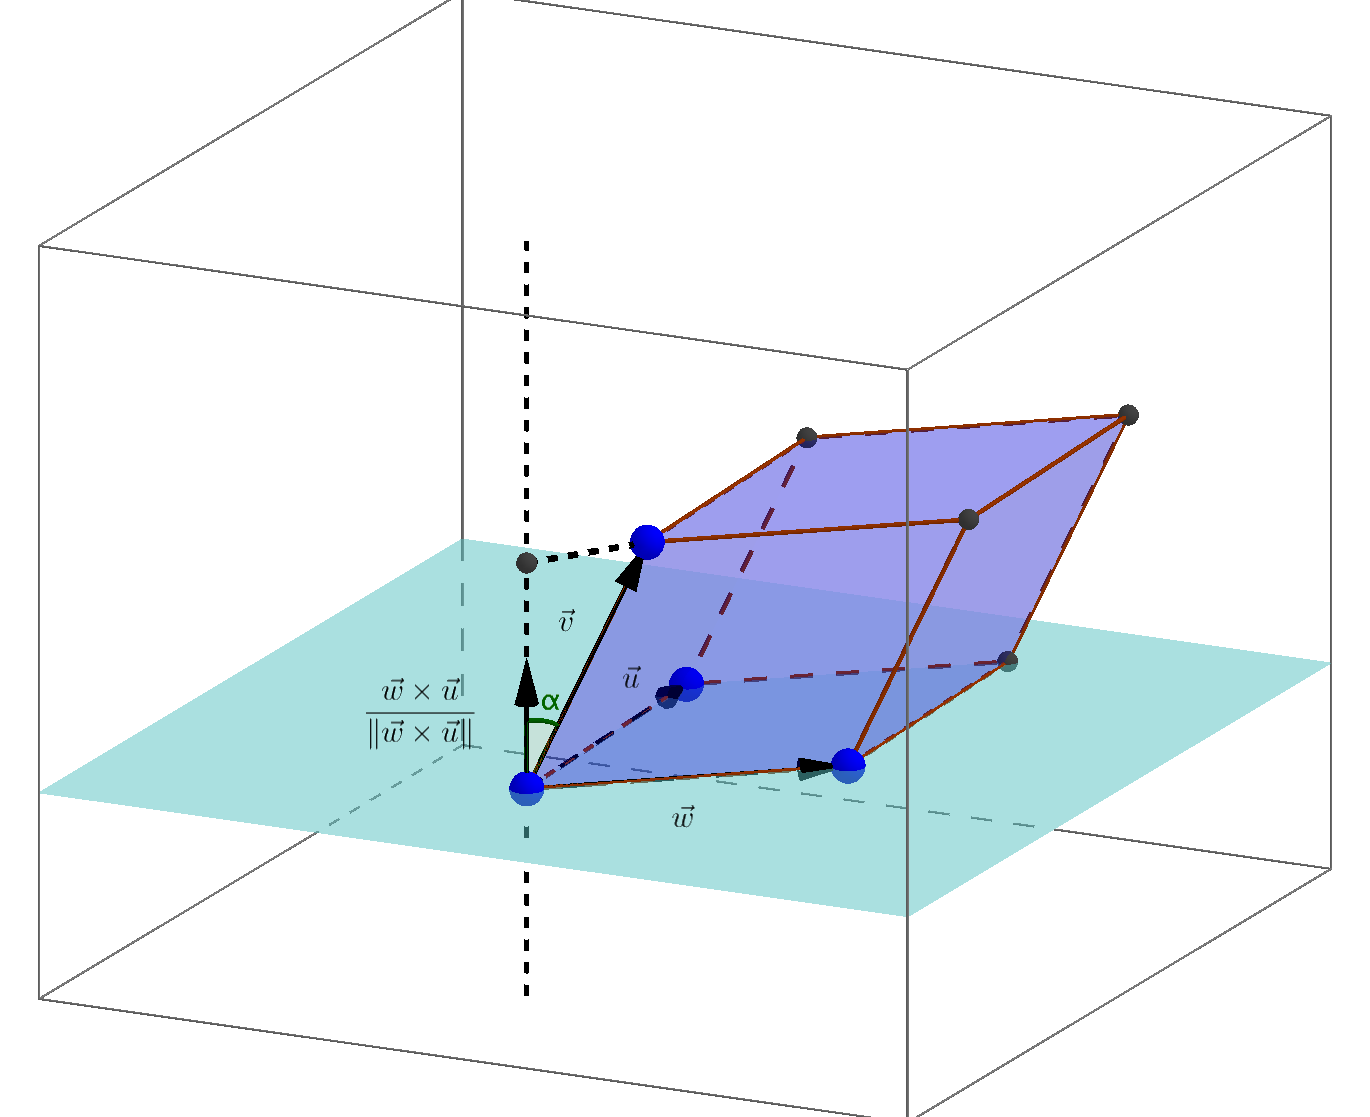
\includegraphics{prodotto_misto}}}
%\put(-132,-5){$\frac{1}{2}$}
%\put(-42,75){$\frac{1}{2}$}
}
\caption{\small Interpretazione geometrica del prodotto misto}%\label{fig:???}
\end{center}
\end{figure}
%%% =======================================================    

\subsection*{Prodotto misto}
In uno spazio euclideo 3--dimensionale \`e definito il prodotto misto ossia un 
prodotto che
coinvolge un prodotto vettoriale e un prodotto misto. Dati tre vettori di $\vec 
v,\vec w\vec z$ 
in $\bE{3}$:
\[
  \vec v\cdot \vec w\times\vec z = \det[\textrm{Col}(\vec v,\vec w, \vec z)]
\]
in cui $\textrm{Col}(\ldots)$ indica la matrice delle colonne dei vettori 
indicati tra parentesi.
Dall'interpretazzione geometrica del prodotto vettoriale e del prodotto scalare 
si 
evince che il $\vec v\cdot \vec w\times\vec z$ sia il volume con segno del 
parallelepipedo di 
spigoli $\vec v,\vec w, \vec z$.

Il prodotto misto, permette quindi di introdurre il concetto di base orientata. 
Una base di 
$\bE{3}$ si dir\`a equiorientata con la base canonica se la sua forma volume 
associata 
\`e positiva. Si osservi che per le propriet\`a del determinante, al variare 
dell'ordine 
degli elementi della base varier\`a anche l'orientazione della stessa.


%\end{document}

%\subsection*{Doppio prodotto vettore}


\section{Rudimenti di Teoria delle curve nello spazio}
Un modo ``semplice'' e naturale per pensare ad una curva consiste 
nell'interpretarla 
come quello strumento che descrive il moto di una particella (o punto 
materiale): 
ad un dato istante $t_1$ la particella si trova nel punto dello spazio 
individuato dalle
coordinate $(x(t_1),y(t_1),z(t_1))$. \`E importante osservare fin da subito che 
l'interesse
non \`e volto solamente alla traiettoria descritta dalle particelle, ma anche 
alle propriet\`a
di questa, ad esempio da {\it come} la traiettoria viene percorsa. 
%%% ========================= FIGURE  ======================
\begin{figure}[h!]
\begin{center}
{\small
{\scalebox{.5}{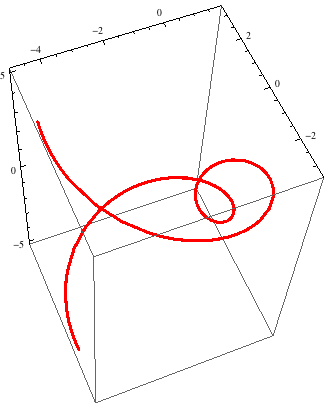
\includegraphics{curva}}}
%\put(-132,-5){$\frac{1}{2}$}
%\put(-42,75){$\frac{1}{2}$}
}
%\caption{\small INTERPRETAZIONE GEOMETRICA DEL PRODOTTO MISTO}\label{fig:???}
\end{center}
\end{figure}
%%% =======================================================      
\begin{definition}
  Una {\bf curva parametrica} in $\bR{n}$ con $n\le 3$\footnote{Pensato come 
spazio affine su se stesso.} 
  \`e una funzione differenziabile 
  \[\begin{aligned}
    \gamma: & \; ]a,b[ \longrightarrow \bR{n}\\
    &\;  t\longmapsto \gamma(t):=(x(t),y(t),z(t))
  \end{aligned}\]
\end{definition}
Una curva quindi \`e individuata da una funzione di un aperto di $\bR{}$ in 
$\bR{n}$.
Dire che $\gamma$ \`e differenziabile per noi significher\`a che $\gamma$ 
ammette 
un numero sufficiente di derivate. Inoltre nel caso di funzioni a valori 
vettoriali, 
la derivazione si effettua per componenti, cio\`e guardando le singole 
componenti 
della funzione come funzioni di variabile reale.
\begin{example}
  Si consideri la curva cartesiana\footnote{Una curva \`e detta cartesiana se si 
pu\`o porre 
  nella forma $\gamma(x) = (x,f(s))$ con $f(x)$ funzione di una variabile.}
  \[\begin{aligned}
    \gamma: & \; ]a,b[ \longrightarrow \bR{2}\\
    &\;  t\longmapsto \gamma(t):= (t,t^2)
  \end{aligned}\]
%%% ========================= FIGURE  ======================
\begin{figure}[h!]
\begin{center}
{\small
{\scalebox{.7}{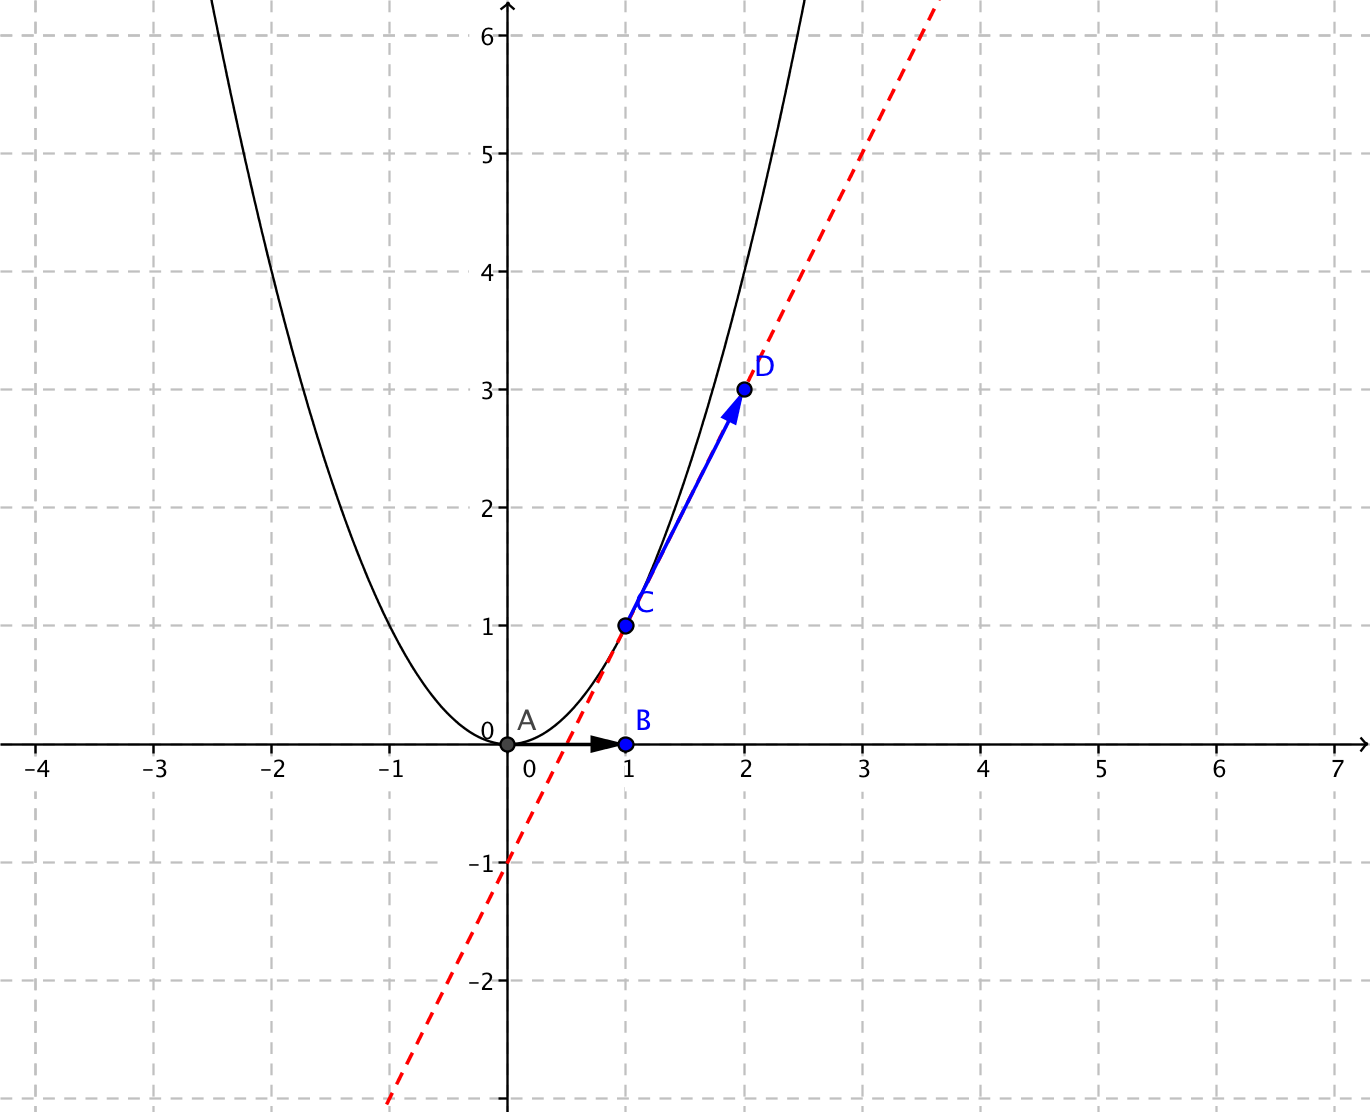
\includegraphics{parabola}}}
%\put(-132,-5){$\frac{1}{2}$}
%\put(-42,75){$\frac{1}{2}$}
}
%\caption{\small INTERPRETAZIONE GEOMETRICA DEL PRODOTTO MISTO}\label{fig:???}
\end{center}
\end{figure}
%%% =======================================================        
  Ora  
  \[
    \dot\gamma(t) = \frac{d}{dt}\, \gamma(t) = \frac{d}{dt}\, (t,t^2) = 
\left(\frac{dt}{dt},\frac{dt^2}{dt}\right)
    = \left(1,2t\right). 
  \]
  $\dot\gamma$ \`e quindi un vettore in $\bR{2}$. $\dot \gamma(t)|_{t=0} = 
(1,0)$ \`e un vettore
  tangente alla curva nel punto in cui esso \`e calcolato. Cos\`{i} 
$\dot\gamma(1) = (1,2)$ 
  \`e un vettore applicato a $\gamma(1) = (1,1)$ e tangente a $\gamma$.   
\end{example}

$\dot\gamma(t)$ \`e un vettore tangente alla curva $\gamma$ nel punto 
$\gamma(t)$: 
per tale ragione \`e detto {\bf vettore velocit\`a}. La norma 
$\|\dot\gamma(t)\|$ di 
$\dot\gamma(t)$ \`e  detta {\bf velocit\`a} della curva. Si noti, come evidente 
anche 
dall'esempio precedente, che generalmente la velocit\`a di una curva varia da 
punto a punto.
(Ci\`o dovrebbe essere immediato se si pensa ad una curva come ad una 
traiettoria
di un moto, infatti in generale un moto non avviene con velocit\`a costante, non 
\`e 
cio\`e uniforme, ma ci sono frenate, accelerazioni, etc.)

\begin{example}
  Si consideri la curva
  \[\begin{aligned}
    \gamma: & \; ]a,b[ \longrightarrow \bR{3}\\
    &\;  t\longmapsto \gamma(t):= (3t^2,2t,1+e^t)
  \end{aligned}\]  
  $\dot\gamma(t) = (6t,2,e^t)$ e $\|\dot\gamma\| = 35t^2+e^{2t}+4$.
  Cio\`e la curva $\gamma$ ha velocit\`a che varia da punto a punto.
\end{example}
Una curva in cui $\|\dot\gamma(t)\}\ne0$ per ogni $t\in]a,b[$ \`e detta {\bf 
regolare}.\\
Per le curve regolari \`e possibile misurare la lunghezza della curva stessa 
abbastanza
semplicemente:
\[
  L[\gamma|^d_c] = \int_c^d \|\gamma(\xi)\| \, d\xi
\]
Il significato geometrico di tale formula \`e abbastanza intuitivo: data una 
curva $\gamma$,
si consideri una suddivisione $\{c=t_0,t_1,\ldots,t_{n-1},t_n=d\}$ 
dell'intervallo $[c,d]$ nel quale si vuole calcolare la lunghezza 
di $\gamma$. Ci\`o permette di definire una spezzata $s(t)$ con i vertici tutti 
in $\gamma$
la cui lunghezza sar\`a
\[
  L[s|_c^d] = \sum_{i=1}^n \| \gamma(t_i)-\gamma(t_{i-1}) \|
\]

%%% ========================= FIGURE  ======================
\begin{figure}[h!]
\begin{center}
{\small
{\scalebox{.7}{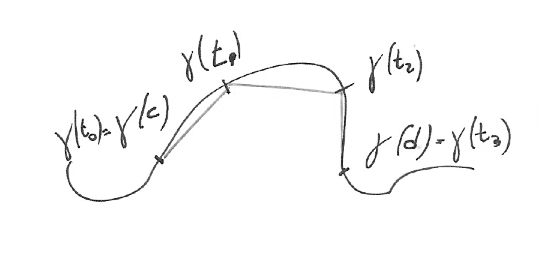
\includegraphics{rettificazione}}}
%\put(-132,-5){$\frac{1}{2}$}
%\put(-42,75){$\frac{1}{2}$}
}
\caption{\small Rettificazione di una curva}\label{fig:???}
\end{center}
\end{figure}
%%% =======================================================    

La spezzata $s(t)$ pu\`o essere pensata come un'approssimazione di $\gamma$, 
quindi 
raffinando la suddivisione, al limite per $i\longrightarrow +\infty$ i segmenti 
$\gamma(t_i)-\gamma(t_{i-1})$ si confonderanno con i vettori tangenti a 
$\gamma$, 
fornendo cos\`{i} la lunghezza di $\gamma$.

\begin{example}
  {\it Si determini la velocit\`a di una curva cartesiana $\gamma(t) = 
(t,f(t))$, con $f(t)$
  funzione reale di variabile reale.}
\end{example}
\begin{sol}
  Il vettore velocit\`a di $\gamma$ \`e $\dot \gamma(t) = \left(1, 
\frac{df(t)}{dt}\right)$. Da cui
  \[
    \|\dot\gamma(t) \| =\sqrt{1+\left(\frac{df(t)}{dt}\right)^2}
  \]
\end{sol}

\begin{example}
  Si consideri 
  \[\begin{aligned}
    \gamma: & \; ]a,b[ \longrightarrow \bR{2}\\
    &\;  \theta\longmapsto \gamma(\theta):= (\cos\theta,\sin\theta)
  \end{aligned}\]
  cerchio unitario di centro l'origine. Calcoliamone la lunghezza.
  \[
    L[\gamma] = \int_0^{2\pi} \|\dot\gamma(\theta)\|\, d\theta = \int_0^{2\pi} 
d\theta = 2\pi
  \]
  essendo $\dot\gamma(\theta) = (-\sin\theta,\cos\theta)$ e quindi 
$\|\dot\gamma(\theta)\|=1$.
\end{example}

\begin{exercise}
  {\it Si determini la velocit\`a di una curva parametrizzata in coordinate 
polari, 
  $x(t)= \rho(t)\cos\theta(t)$, $y(t)= \rho(t)\sin\theta(t)$, con 
$(\rho,\theta)\in \bR{*}_+\times]0,2\pi[$.}
\end{exercise}

Si osservi che differenti curve possono avere la medesima traccia e viceversa. 
Per studiare ci\`o, ma in generale anche da un punto di vista meccanico, \`e 
utile considerare riparametrizzazioni di curve. 
\begin{definition}
  Sia $\gamma:]a,b[\longrightarrow \bR{3}$ una curva parametrica e sia 
  $\phi:]a,b[ \longrightarrow]c,d[$ una funzione continua, invertibile con 
  inversa continua\footnote{Cio\`e $\phi$ sia un omeomorfismo.} La funzione
  $\delta: ]c,d[\longrightarrow\bR{3}$ \`e una {\bf riparametrizzazione} di 
$\gamma$
  (e viceversa) se 
  \[
    \gamma = \delta\circ\phi
  \]
  
%%% ========================= FIGURE  ======================
\begin{figure}[h!]
\begin{center}
{\small
{\scalebox{.55}{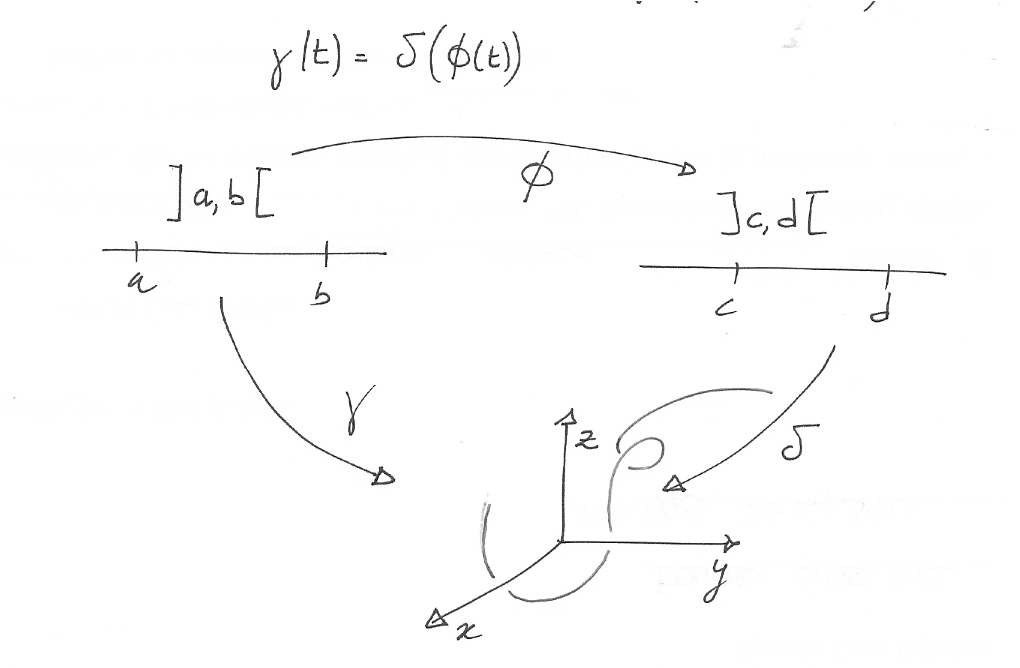
\includegraphics{riparametrizzazione}}}
%\put(-132,-5){$\frac{1}{2}$}
%\put(-42,75){$\frac{1}{2}$}
}
%\caption{\small INTERPRETAZIONE GEOMETRICA DEL PRODOTTO MISTO}\label{fig:???}
\end{center}
\end{figure}
%%% =======================================================      
  
\end{definition}
\begin{example}
  Si considerino le curve $\gamma: \;t\in]0,2\pi[\longrightarrow (\cos t,\sin 
t)\in\bR{2}$ 
  e $\delta:\;\tau\in ]0,\pi[\longrightarrow (\cos2\tau,\sin2\tau)\in\bR{2}$. La 
traccia di 
  entrambe le curve \`e una circonferenza di raggio 1 e centro l'origine. La 
differenza 
  tra le due curve consiste nella velocit\`a di percorrenza, infatti 
$\|\dot\gamma\|=1$
  e $\|\dot \delta\|=2$: $\delta$ percorre il supporto a velocit\`a doppia di 
$\gamma$.
  Si noti che entrambe le curve sono percorse con velocit\`a uniforme, pertanto 
\`e
  semplice immaginare che le due curve siano una riparametrizzazione una 
dell'altra.
  La funzione $\phi:]0,\pi[\ni t \longrightarrow ]0,\pi/2[\ni \tau:=t/2$.
\end{example}

\newpage

{\small
\begin{thebibliography}{99}

\bibitem[Candilera]{C} M. Candilera, {\it Dispensa di Geometria.} Reperibile 
alla pagina web 
http://www.math.unipd.it/~candiler/mat\_tre.html

\bibitem[Cornalba]{Cor} M. Cornalba {\it Piccola introduzione alla geometria 
proiettiva.}
Reperibile alla pagina web \\
http://mate.unipv.it/cornalba/dispense/proj.pdf

\bibitem[Sernesi]{Ser} E. Sernesi, {\it Geometria 1.} Bollati Boringhieri.

\bibitem[Spera--1]{Sp1} M. Spera, {\it Note di Elementi di Geometria.} Non 
pubblicate.

\bibitem[Spera--2]{Sp2} M. Spera, {\it Note del Corso di Geometria.} Libreria 
Progetto.

\bibitem[Spera--3]{Sp3} M. Spera, {\it Note di Geometria Computazionale.} Non 
pubblicate.

\bibitem[Spera--4]{Sp4} M. Spera, {\it Comunicazioni private.}


\end{thebibliography}
}


\end{document}

\section*{Appendice}

\begin{center}\textcolor[rgb]{0.50,0.20,0.50}{\bf MONA.} \end{center}

\textcolor{blue}{\begin{NB}
  MINNI
\end{NB}}

\begin{comment}  
  \begin{itemize}
  \item {\it {\small PIPPO 
  \item PLUTO}}
  \end{itemize}
\end{comment}


%\begin{exercise}
  
%\end{exercise}



\end{document} 

%%% ========================= FIGURE  ======================
\begin{figure}[h!]
\begin{center}
{\small
{\scalebox{1.}{\includegraphics{homotopy2}}}
\put(-132,-5){$\frac{1}{2}$}
\put(-42,75){$\frac{1}{2}$}
}
\caption{\small }\label{fig:quadrato2}
\end{center}
\end{figure}
%%% =======================================================  


\noindent
{\bf N.B.}\\
Il simbolo $\blacksmiley$ denota esercizi giudicati \textcolor{red}{\bf 
difficile}.

\section{I primi teoremi}
\label{sec:3D_teoremi}

\section{...}
\label{sec:3D_...}


